\subtitlepage{SaltStack}{Ещё кое-что}

\begin{Frame}{Пишем модули}
  \framesubtitle{Особенности}

  \begin{center}
    Все мы в душ\'е немного программисты \inlineicon{\faKeyboard[regular]}
  \end{center}

  \onslide<+->

  \begin{itemize}[<+-| alert@ +>]
    \setbeamertemplate{itemize item}{\faCode}

    \item[\faPython] Python\vfill
    \item[{\faHandshake[regular]}] Единые соглашения для разных модулей\vfill
    \item[\faHatWizard] Различающийся контекст
    \item[\faMicroscope] Работает через интроспекцию
    \item[\faSkullCrossbones] Аннотирование типов ломает интроспекцию
  \end{itemize}

  \vfill

  \onslide<+->
  \begin{center}
    \inlineicon{\faLightbulb[regular]}
    Не забываем \texttt{salt '*' saltutil.sync\_all}
  \end{center}

  \overlaypic{south east}{width=75pt}{snake}
\end{Frame}

\begin{frame}{Пишем модули}
  \framesubtitle{Соглашения}

  \ExampleNote{}

  \begin{itemize}[<+-| alert@ +>]
    \setbeamertemplate{itemize item}{\faCode}
    \item Ищутся любые подходящие функции
    \item Функции возвращают словари
    \item \texttt{\_\_virtual\_\_: function}
    \item \texttt{\_\_init\_\_: function}, получающая настройки миньона
    \item \texttt{\_\_salt\_\_: dict}\footnote{%
      На деле \texttt{NamedLoaderContext} \faGhost}
    \item \texttt{\_\_virtualname\_\_: str}
    \item \texttt{\_\_func\_alias\_\_: dict}
  \end{itemize}
\end{frame}

\liveframe{}

\begin{Frame}{Реакторы}

  \ExampleNote{}

  \begin{itemize}[<+-| alert@ +>]
    \item Действие по событию (как callback)
    \item Прописываются последовательностью в конфиге мастера
    \item Сопоставляют действие тэгу события
    \item Бывают local, runner, wheel и caller
    \item Переменные Jinja доступны ограниченно, реквизитов нет
    \item[\faTerminal] \texttt{salt-run event.send ТЭГ СЛОВАРЬ} для отладки
  \end{itemize}

  \vfill

  \centering
  
\includegraphics[width=75pt]{iso-radiation}
\end{Frame}

\liveframe{}

\Setsubsection{Шедулинг}
\begin{frame}[fragile]
  \frametitle{\Insertsubsection}

  \begin{itemize}[<+-| alert@ +>]
    \setbeamertemplate{itemize items}{\faClock[regular]}

    \item Похоже на cron или systemd.timer
    \item Прописывается в конфиге миньона или мастера
    \item Запуск модулей, применение состояний
    \item На миньоне модули исполнения, на мастере модули раннеров
  \end{itemize}

  \onslide<+->
  \begin{center}\begin{minipage}{0.4\textwidth}
    \begin{minted}[gobble=6]{yaml}
      schedule:
        write_to_file:
          function: cmd.run
          seconds: 5
          args:
            - 'date >> /tmp/salt.log'
          kwargs: {}
          splay: 3
    \end{minted}
  \end{minipage}\end{center}
\end{frame}

\liveframe{}

\begin{Frame}{В двух словах о Salt Mine}
  \begin{itemize}[<+-| alert@ +>]
    \item Шахты похожи на грейны
    \item Значения доступны для миньонов
    \item Можно настроить в конфиге миньона
    \item Можно настроить в пилларах
    \item Для получения значений \texttt{mine.get}
    \item[\faAngleDoubleRight] Пример в следующей секции
  \end{itemize}
\end{Frame}

\begin{Frame}{Оркестрация}
  \framesubtitle{Это\dots}

  \ExampleNote{}

  \begin{itemize}[<+-| alert@ +>]
    \item[\faRunning] Salt Orchestration Runner
    \item[\faMountain] Выше, чем highstate
    \item[\faBullhorn] Вызовы функций для управления инфраструктурой
    \item[\faTerminal] \texttt{salt-run state.orchestrate SLS\_ФАЙЛ}
  \end{itemize}
\end{Frame}

\begin{frame}{Оркестрация}
  \framesubtitle{Матрёшка}
  \centering
  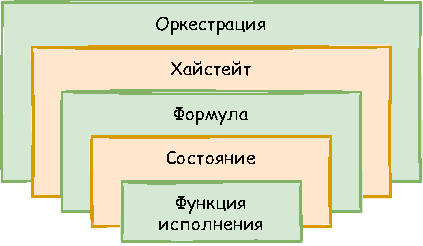
\includegraphics[width=0.5\textwidth]{saltstack-matryoshka}
  \overlaypic{south east}{width=140pt}{matryoshkas}
\end{frame}

\liveframe{}

\begin{Frame}{Salt Cloud}
  \begin{itemize}[<+-| alert@ +>]
    \item[\faCloud] Провиженинг виртуальных машин
    \item[\faCogs] Куча коннекторов\footnote<2->{Но не для отечественных
      \faCloud\faCloud\faMeh[regular]}
    \item[{\faFileCode[regular]}] Определяем провайдера и профиль машины
    \item[\faServer] Элегантно разворачиваемся
    \item[{\faMap[regular]}] mapfile для подхода <<инфраструктура как код>>
  \end{itemize}
\end{Frame}

\begin{frame}{Salt Cloud}
  \framesubtitle{Команда}

  \ExampleNote{}

  \setbeamertemplate{itemize item}{\faTerminal}

  \begin{itemize}[<+->]
    \item \texttt{salt-cloud [-P] -p ПРОФИЛЬ ИМЯ\_1 ИМЯ\_2 \ldots\ ИМЯ\_N} \\
      \color{Gray} \small Создать машины из профиля (\texttt{-P} --- параллельно)

    \vfill

    \item \texttt{salt-cloud [-P] -m МАПФАЙЛ} \\
      \color{Gray} \small Создать машины по карте

    \vfill

    \item \texttt{salt-cloud -m МАПФАЙЛ -d} \\
      \color{Gray} \small Удалить машины, указанные в карте

  \end{itemize}
\end{frame}

\liveframe{}

\begin{Frame}{Ссылки на документацию}

  \vfill
  \begin{itemize}
    \setbeamertemplate{itemize item}{\faLink}
    \item \uhref{%
      https://docs.saltproject.io/en/latest/topics/development/modules/developing.html}{%
      Разработка модулей}\vfill

    \item \uhref{%
      https://docs.saltproject.io/en/latest/topics/reactor/index.html}{%
      Реакторы}\vfill

    \item \uhref{%
      https://docs.saltproject.io/en/latest/topics/jobs/index.html\#scheduling-jobs}{%
      Планируемые задачи}\vfill

    \item \uhref{%
      https://docs.saltproject.io/en/latest/topics/orchestrate/orchestrate_runner.html}{%
      Оркестрация}\vfill

    \item \uhref{%
      https://docs.saltproject.io/en/latest/topics/cloud/index.html}{%
      Salt Cloud}\vfill
  \end{itemize}
\end{Frame}

% vi: ft=tex
